\section{Resultados}
Una vez concluido el análisis cualitativo, se determinó que el desarrollo de un sistema moderno requiere apoyarse en una combinación equilibrada de herramientas, metodologías y lenguajes que aseguren organización, escalabilidad y colaboración efectiva. En este sentido, se confirmó la relevancia de contar con un control de versiones robusto mediante Git y GitHub, así como de aplicar un marco ágil bien estructurado como la Guía de Scrum 2020, que permite adaptarse a los cambios, mejorar la comunicación entre los participantes y facilitar la entrega incremental de funcionalidades. Estos hallazgos orientaron las decisiones técnicas adoptadas y proporcionaron lineamientos prácticos para optimizar el trabajo en equipo y la calidad del producto final.

\subsection{Resultados en la arquitectura y el desarrollo del sistema}
Se implementó un software basado en el patrón Modelo–Vista–Controlador (MVC), el cual facilitó una clara separación de responsabilidades entre la lógica de negocio, la interfaz de usuario y la gestión de las interacciones. De forma complementaria, la aplicación de patrones de diseño aportó soluciones comprobadas para problemas comunes, incrementando la reutilización y la flexibilidad de la estructura. El lenguaje Java, elegido como núcleo del desarrollo, ofreció robustez, portabilidad y un amplio ecosistema de librerías, mientras que el uso de Git y GitHub garantizó la trazabilidad de los cambios y la colaboración distribuida del equipo. En conjunto, estos elementos permitieron construir un sistema escalable, seguro y alineado con las mejores prácticas del desarrollo de software contemporáneo.

\begin{figure}[htbp]
    \centering
    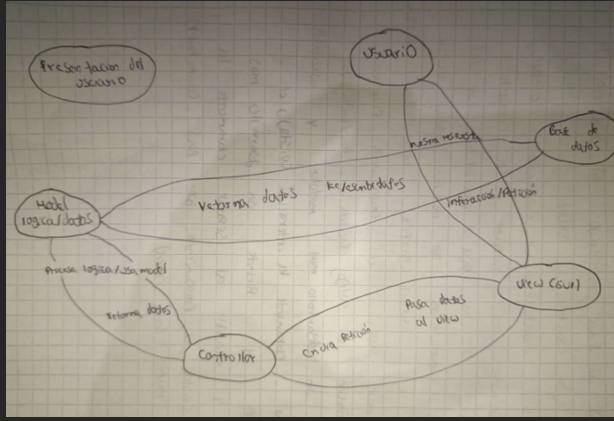
\includegraphics[width=0.5\textwidth]{graphics/MVC-patron.png}
    \caption{Modelo vista controlador}
    \label{fig:mvc}
\end{figure}

En la Figura \ref{fig:mvc} se presenta el diagrama de la arquitectura Modelo–Vista–Controlador (MVC) utilizada en el desarrollo del sistema. Esta representación muestra la interacción entre el Modelo, que gestiona la lógica de datos, el Controlador, encargado de coordinar las solicitudes del usuario, y la Vista, responsable de la presentación. El uso de MVC favoreció una organización clara del código y facilitó la incorporación de nuevas funcionalidades, permitiendo que las actualizaciones en cada componente se realicen sin afectar de manera negativa al resto de la aplicación.

\subsection{Resultados en la aplicación de la metodología ágil (Scrum)}
Durante el año académico se aplicaron los principios de Scrum en tres proyectos diferentes, manteniendo un registro continuo de avances y evidencias que demuestran la participación activa en cada uno de ellos. A continuación, se detallan los aportes y las pruebas de trabajo:

• \textbf{Odimo – Plataforma de domicilios}

Rol y aportes: desarrollo del backend, diseño de mockups en Figma y elaboración de documentación.

Evidencias: repositorio en GitHub con commits de las funcionalidades implementadas y material de soporte en Microsoft Teams.

URL de evidencia:

Github: \url{https://github.com/Darwin-9/Odimo.git}

Figma: \url{https://www.figma.com/design/lmqPj5pLqUQrRX6R1vQPms/Untitled?node-id=0-1&t=up4yA4ZGq39i7p2n-1}

Teams-Documentación: ADSO 2899747 - Documents - Soporte - All Documents

• \textbf{Sistema de Gestión de Inventario}

Rol y aportes: finalización de la documentación, desarrollo del backend funcional y comienzo del frontend, además de algunos mockups.

Evidencias: código y commits en GitHub, así como archivos de prueba y avances documentados en Microsoft Teams.

URL de evidencia:

Github: \url{https://github.com/Darwin-9/InventorySystem.git}

Figma: \url{https://www.figma.com/design/V89kbquYJic3yF700ZFP2K/Untitled?node-id=0-1&t=Y1Rj5pGSEjQQrcCH-1}

Teams-Documentación: Grupo 8- Gestión de Inventario ODIMO CANCELADO

• \textbf{Tu-Evento – Proyecto actual}

Rol y aportes: contribuciones activas en documentación, código y mockups, evidenciadas por los commits realizados y el trabajo colaborativo con el equipo.

Evidencias: historial de commits en GitHub y material compartido con los compañeros que confirma la participación en las diferentes fases del proyecto.

URL de evidencia:

Github: \url{https://github.com/lozano2303/tu-evento.git}

Figma: \url{https://www.figma.com/design/iuw3YMS7t81m3hIKMAvtHf/Tu-Evento?node-id=0-1&t=kUGHUgTCtokrMqo6-1}

Teams-Documentación: Grupo 5- Tu evento

\begin{figure}[htbp]
    \centering
    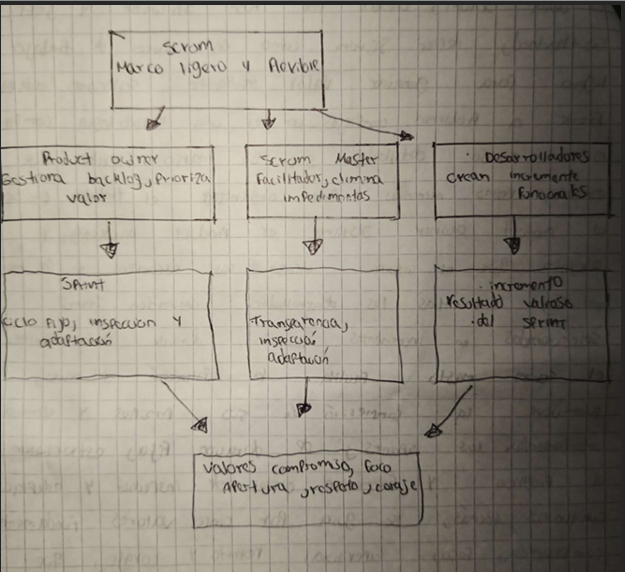
\includegraphics[width=0.5\textwidth]{graphics/scrum.png}
    \caption{Evidencias de trabajo colaborativo}
    \label{fig:evidencias}
\end{figure}

En la Figura \ref{fig:evidencias} se presentan las principales plataformas que sirvieron como soporte para la planificación, el seguimiento de avances y la entrega de resultados en los tres proyectos desarrollados durante el año. En lugar de un tablero de Trello, la organización y control de tareas se documentaron directamente en GitHub, Figma y Microsoft Teams, donde se registran commits, diseños, documentación y mensajes de comunicación del equipo.